\documentclass[a4paper, 12pt]{article}
\usepackage[T1]{fontenc}
\usepackage[utf8]{inputenc}

% \usepackage[ngerman]{babel} % for German, before newpx
\usepackage{mathtools} % loads and fixes ams, mathclap, coloneqq, text over arrows, etc
\usepackage[amsthm]{newpx} % loads amsmath

% \usepackage{amssymb} % for \mathbb, \mathcal
% \usepackage{amsthm} % for theorem environments

\usepackage{csquotes} % for \enquote
\usepackage{braket} % for \bra, \ket, \braket
\usepackage{quantikz} % for quantum circuits
\usepackage{parskip} % for no paragraph indentation
\usepackage{enumitem} % for custom enumeration labels
% \usepackage{wasysym}  % for \Lightning symbol
\usepackage{ marvosym }
\usepackage{bm} % for bold math symbols
\usepackage{graphicx} % for images
\usepackage{newpx} % Palatino font
\usepackage{geometry} % better margins

\theoremstyle{plain}
\newtheorem*{theorem}{Theorem}
\newtheorem*{lemma}{Lemma}
\newtheorem*{corollary}{Corollary}

\theoremstyle{definition}
\newtheorem*{definition}{Definition}
\newtheorem*{example}{Example}

\theoremstyle{remark}
\newtheorem*{note}{Note}
\newtheorem*{observation}{Observation}

\date{\today}

\renewcommand{\H}{\mathcal{H}}
\newcommand{\C}{\mathbb{C}}

\DeclareMathOperator{\tr}{tr}

\begin{document}
\begin{titlepage}
  \centering
  \vspace*{0.06\textheight}
  {\large Norbert Schuch}\\[\baselineskip]
  {\Huge QUANTUM ERROR}\\[\baselineskip]
  % {\Large and}\\[\baselineskip]
  {\Huge CORRECTION}\\[\baselineskip]
  {\small\scshape Wintersemester 2024}\\[\baselineskip]
  {\scshape Transcribed and Typeset by}\\
  % {\scshape }\\
  {\large\scshape Maximilian Fettinger}\\[2\baselineskip]
  {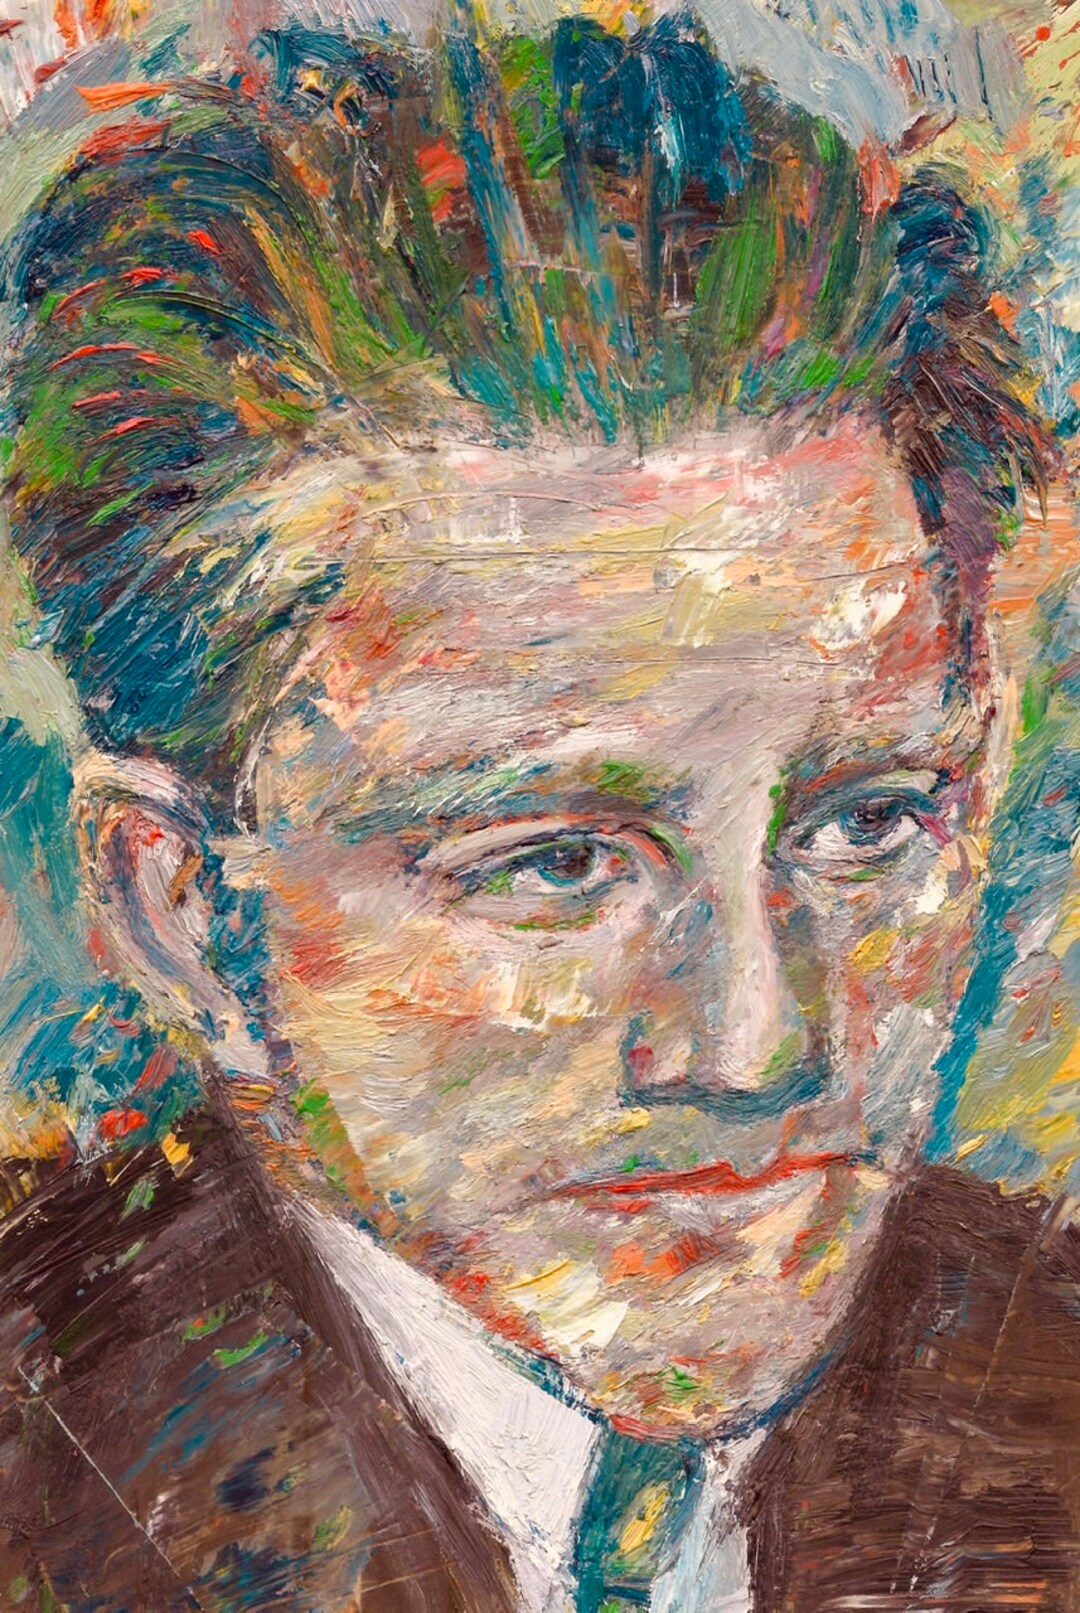
\includegraphics[width=0.3\textwidth]{heisenberg.png}}\\[\baselineskip]
  {\small\scshape University of Vienna}\par
  \vfill\null
\end{titlepage}

\section{Introduction}
\subsection{Setting and Problem}

\begin{itemize}
  \item Coupling to \textbf{environment} induces \textbf{errors}
  \item Classical computer: Information stored in \emph{macroscopic} properties $\rightarrow$ errors unlikely
  \item Quantum computers:
    \begin{itemize}
      \item need qubits = \emph{single} quantum systems, and must store general superpositions, not just $\ket{0}$ and $\ket{1}$ $\rightarrow$ \textbf{fragile!}
      \item should be well isolated to protect qubits, but also need coupling to \emph{environment} (experimental apparatus) to control the computation (gates, measurements).
    \end{itemize}
\end{itemize}

\textbf{Question:} Can we protect quantum information from noise?
\subsubsection*{Classical Error Correction}
\textbf{Copy} information (\emph{encoding}), e.g encode 1 bit in 3 bits:
\begin{align*}
  0 &\mapsto \hat{0} \coloneqq 000 \\
  1 &\mapsto \hat{1} \coloneqq 111
\end{align*}

\textbf{Error Model:} Bit flip with some (small) probability $p$ (independently for all bits) $\Longrightarrow$ typically 0 or 1 bits flipped.

Error correction (\emph{decoding}) by majority vote:
\begin{align*}
  000, 001, 010, 100 &\mapsto 000 \\
  111, 110, 101, 011 &\mapsto 111
\end{align*}

Probability for a \emph{\textbf{logical error}} (i.e. on encoded bit):
\begin{align*}
  p_{\text{error}} &= \Pr(\geq 2 \text{ flips}) = p^3 + 3p^2(1-p) \\
  &= 3p^2 - 2p^3 < p \quad \text{for } p < \frac{1}{2}
\end{align*}
Error quadratically suppressed $\rightarrow$ effective error probability \textbf{decreased}.

Can be improved by:
\begin{itemize}
  \item using more bits: $0 \mapsto 00\ldots0, 1 \mapsto 11\ldots1$
  \item nesting (\emph{concatenating}) codes
  \item using smarter codes (i.e encode several bits at once)
\end{itemize}
\subsubsection*{Quantum Error Correction}
Several potential problems when trying to generalize classical error correction codes:
\begin{itemize}
  \item cannot copy qubits
  \item even if we could: what would be the \emph{majority vote}?
  \item \textbf{different types of errors} exist, e.g. X (bit flip) or Z (phase flip)
  \item errors can be continuous: there is an \textbf{infinity} of errors!
  \item measuring qubits \textbf{destroys} quantum information!
\end{itemize}

\subsection{The 3-qubit bit flip code}
Copy qubits in computational basis:
\begin{align*}
  \ket{0} &\mapsto \ket{\hat{0}}=\ket{000} \\
  \ket{1} &\mapsto \ket{\hat{1}}=\ket{111}
\end{align*}
i.e., the encoding is a linear map
\begin{equation*}
  \ket{\psi} = \alpha\ket{0} + \beta\ket{1} \xmapsto{\text{encoding}} \alpha\ket{000} + \beta\ket{111}
\end{equation*}

Possible \textbf{encoding circuit}:

\begin{center}
  \begin{quantikz}
    \lstick{$\ket{\psi}$} & \ctrl{1} & \ctrl{2} & \qw & \rstick[3]{$\ket{\hat{\psi}} = \alpha\ket{000} + \beta\ket{111}$} \\
    \lstick{$\ket{0}$}   & \targ{}  & \qw      & \qw &\\
    \lstick{$\ket{0}$}   & \qw      & \targ{}  & \qw &
  \end{quantikz}
\end{center}

Now consider \textbf{bit flip error} on qubit $i$:
\begin{equation*}
  \ket{\hat{\psi}} \xmapsto{\text{error}} X_i \ket{\hat{\psi}}
\end{equation*}

Can we \textbf{correct} for one \textbf{bit flip error} on an unknown qubit $i$?

\textbf{Problem:} Measuring the qubits in computational basis reveals $i$, but also \textbf{destroys superposition!}

$\Longrightarrow$ Need a measurement which \textbf{only} returns information about \textbf{position $i$ of error} -- independently of encoded state $\ket{\psi}$!

Define \emph{syndrome measurement} with outcomes 0, 1, 2, 3, and projectors:
\begin{align*}
  &\text{\textbf{0 = \emph{no flip}:}} &\quad P_0 = \ket{000}\bra{000} + \ket{111}\bra{111} \\
  &\text{\textbf{1 = \emph{1st qubit gets flipped}:}} &\quad P_1 = \ket{100}\bra{100} + \ket{011}\bra{011}\\
  &\text{\textbf{2 = \emph{2nd qubit gets flipped}:}} &\quad P_2 = \ket{010}\bra{010} + \ket{101}\bra{101} \\
  &\text{\textbf{3 = \emph{3rd qubit gets flipped}:}} &\quad P_3 = \ket{001}\bra{001} + \ket{110}\bra{110}
\end{align*}

(This defines a complete measurement, as $\sum_i P_i = I$)

The outcome is called the \emph{error syndrome}.

Measurement of $\{P_\alpha\}$ reveals only \textbf{2 bits of information} $\Longrightarrow$ one qubit of information \textbf{untouched}!

By direct inspection: The information obtained is the location of the bit flip, e.g.
\begin{equation*}
  \alpha \ket{000} + \beta \ket{111} \xmapsto[\text{on qubit 2}]{\text{bit flip}} \alpha \ket{010} + \beta \ket{101}
\end{equation*}

$\Longrightarrow$ measurement always returns $P_2$, with post-measurement state
\begin{equation*}
  \alpha \ket{010} + \beta \ket{101} \xmapsto[\text{flip qubit 2}]{\text{recovery:}}\alpha \ket{000} + \beta \ket{111}\!
\end{equation*}

$\Longrightarrow$ Bit flip \textbf{corrected}!

Works for any simple bit flip in unknown location and no flip, and for all states $\ket{\psi}$.

$\Longrightarrow$ suppression of error $p \rightarrow 3p^2 - 2p^3$, as classically.

By linearity, this also works for part of a larger entangled state:
\begin{multline*}
  \alpha\ket{0}\ket{a}+\beta\ket{1}\ket{b} \xmapsto{\text{encode}} \alpha\ket{000}\ket{a}+\beta\ket{111}\ket{b} \\
  \xmapsto[X_1]{\text{error}}\alpha\ket{100}\ket{a}+\beta\ket{011}\ket{b} \xmapsto[\text{correct: }X_1]{\text{meas.: }P_1}\alpha\ket{000}\ket{a}+\beta\ket{111}\ket{b}
\end{multline*}

What about \textbf{continuous errors}, e.g.
\begin{equation*}
  \ket{\hat{\psi}} \mapsto e^{i \vartheta X_1} \ket{\hat{\psi}} = (\cos \vartheta I + i \sin \vartheta X_1) \ket{\hat{\psi}} ?
\end{equation*}

\begin{align*}
  \ket{\hat{\psi}} &= \alpha\ket{000} + \beta\ket{111} \xmapsto[\text{e.g. }X_3]{\text{error}}
  \alpha (\cos \vartheta \ket{000} + i\sin\vartheta \ket{001})+\beta(\cos \vartheta \ket{111} + i \sin \vartheta \ket{110})\\
  &= \cos \vartheta\underbrace{(\alpha\ket{000} + \beta\ket{111})}_{\text{syndrome } P_0} + i\sin\vartheta \underbrace{(\alpha\ket{001} + \beta\ket{110})}_{\text{syndrome } P_3}
\end{align*}

\textbf{Syndrome measurement collapses state} into:

Prob.: $|\cos\vartheta|^2$: \\result $P_0$, post-measurement state $\alpha\ket{000} + \beta\ket{111}, 0 \equiv \text{no correction:}$ \checkmark

Prob.: $|\sin\vartheta|^2$: \\result $P_3$, post-measurement state $\alpha\ket{001} + \beta\ket{110}, 3 \equiv \text{correction: flip bit 3:}$
$\Rightarrow \alpha \ket{000} + \beta \ket{111}$: \checkmark

Measurement of error syndrome ${P_\alpha}$ collapses \textbf{continuous error} into one of the 4 \textbf{discrete errors}:
\begin{itemize}
  \item measurement \emph{digitalizes} error
  \item sufficient to study discrete (distinguishable) errors (will be formalized later)
\end{itemize}

We have focused on X errors, but what about \textbf{Z errors}?
\begin{equation*}
  \alpha \ket{000} + \beta \ket{111} \xmapsto[\text{on qubit 1}]{Z \text{ error}} \alpha \ket{000} - \beta \ket{111}
\end{equation*}

This is still a state in the \textbf{code space} (i.e. a valid encoded state $\ket{\hat{\psi}}$)

$\Longrightarrow$ error \textbf{not detectable}, but it \textbf{has changed} $\ket{\hat{\psi}}$. After decoding, the error acts as
\begin{equation*}
  \alpha \ket{0} + \beta \ket{1} \mapsto \alpha \ket{0} - \beta \ket{1},
\end{equation*}
i.e. as a \textbf{logical Z operation} (\emph{logical operator} = operation on encoded qubit).

$\Longrightarrow$ 3-qubit bit flip code \textbf{cannot protect against} single \emph{\textbf{phase flip error}} $Z_i$.

\subsection{The 3-qubit phase flip code}

Can we correct against Z errors?
\begin{equation*}
  Z \ket{+} = \ket{-},\, Z \ket{-} = \ket{+}
\end{equation*}

$\Longrightarrow$ Z error $\hat{=}$ bit flip error in $\ket{\pm}$-basis.

Use encoding $\alpha \ket{0} + \beta \ket{1} \mapsto \alpha \ket{\hat{0}}+\beta\ket{\hat{1}}$, with $\ket{\hat{0}} \coloneqq \ket{+++}$, $\ket{\hat{1}} \coloneqq \ket{---}$:

Will protect against single Z errors!

\textbf{Encoding:}
\begin{center}
  \begin{quantikz}
    \lstick{$\ket{\psi}$} & \ctrl{1} & \ctrl{2} & \qw & \gate{H} &\\
    \lstick{$\ket{0}$}    & \targ{}  & \qw      & \qw & \gate{H} &\\
    \lstick{$\ket{0}$}    & \qw      & \targ{}  & \qw & \gate{H} &
  \end{quantikz}
\end{center}

\textbf{Syndrome measurement}:
\begin{equation*}
  \tilde{P}_\alpha = H^{\otimes 3} P_\alpha H^{\otimes 3}
\end{equation*}

\textbf{Recovery operation}:
\begin{equation*}
  H X_i H = Z_i
\end{equation*}

\textbf{Problem:} Now there is no protection against bit flip errors $X_i$ -- and $X_i$ acts as a logical Z operator!

\section{The 9-qubit Shor code}
\textbf{Solution:} Concatenate (= nest) 3-qubit bit flip code and 3-qubit phase flip code:
\begin{align*}
  \ket{0} &\mapsto \ket{+}\ket{+}\ket{+} \mapsto \frac{(\ket{000}+\ket{111})(\ket{000}+\ket{111})(\ket{000}+\ket{111})}{2\sqrt{2}} \\
  \ket{1} &\mapsto \ket{-}\ket{-}\ket{-} \mapsto \frac{(\ket{000}-\ket{111})(\ket{000}-\ket{111})(\ket{000}-\ket{111})}{2\sqrt{2}}
\end{align*}

Encoding circuit:
\begin{center}
  \begin{quantikz}
    \lstick{$\ket{\psi}$} & \ctrl{3}          &\ctrl{6} & \gate{H} & \ctrl{1} & \ctrl{2} &\\
    &\wireoverride{n} &\wireoverride{n}& \wireoverride{n}\lstick{$\ket{0}$} & \targ{} && \\
    &\wireoverride{n} &\wireoverride{n}& \wireoverride{n}\lstick{$\ket{0}$} & & \targ{}&\\
    \lstick{$\ket{0}$}    & \targ{} && \gate{H} & \ctrl{1} & \ctrl{2} &\\
    &\wireoverride{n} &\wireoverride{n}& \wireoverride{n}\lstick{$\ket{0}$} & \targ{} && \\
    &\wireoverride{n} &\wireoverride{n}& \wireoverride{n}\lstick{$\ket{0}$} & & \targ{}&\\
    \lstick{$\ket{0}$}    &                   &\targ{} & \gate{H} & \ctrl{1} & \ctrl{2} &\\
    &\wireoverride{n} &\wireoverride{n}& \wireoverride{n}\lstick{$\ket{0}$} & \targ{} && \\
    &\wireoverride{n} &\wireoverride{n}& \wireoverride{n}\lstick{$\ket{0}$} & & \targ{}&\\
  \end{quantikz}
\end{center}

Shor code protects against \textbf{arbitrary} single qubit errors! Sufficient to focus on X, Z, and $Y \propto XZ$ errors:

Any general error $E = \alpha I + \sum_i \beta_i \sigma_i$ will collapse to one of those (if done right).

--- More on this later! ---

\textbf{Intuitively:}
\begin{enumerate}[label=(\roman*)]
  \item Errors $X_i$ are corrected on \emph{inner code} layer.
  \item $Z_i$ error = \\
    = \textbf{logical} error on qubit encoded in inner layer\\
    = Z error on outer layer in one position\\
    $\Longrightarrow$ correctable!
  \item $Y_i \propto X_i Z_i$: \\correct $X_i$ on inner layer, then as in (ii): only Z error left!
\end{enumerate}

What if errors occur on \textbf{more than one qubit}?

Some -- but not all! -- can be corrected, e.g.
\begin{align*}
  X_1 X_4&: \text{ correctable} \\
  Z_1 Z_2&: \text{ trivial = no error} \\
\end{align*}
but:
\begin{align*}
  X_1 X_2&: \text{ breaks inner code \Lightning}\\
  Z_1 Z_4&: \text{ breaks outer code \Lightning}
\end{align*}

\section{The Quantum Error Correction Conditions}
\begin{definition}
  Given $\H = (\C^2)^{\otimes n}$, a \textbf{quantum error correction code (QECC)} on $\H$ is a subspace $\mathcal{C} \subset \H$ (the \textbf{code space}, with $\ket{\psi} \in \mathcal{C}$ \textbf{codewords}). We denote by $\ket{\hat{\imath}}$ an (arbitrary, but fixed) basis of $\mathcal{C}$.
\end{definition}

\begin{definition}
  A \textbf{noise model} on $\H$ is a CP map
  \[
    \mathcal{E}(\rho) = \sum E_\alpha \rho E_\alpha^\dagger; \quad \sum E_\alpha^\dagger E_\alpha \leq I
  \]
  (i.e., error $E_\alpha$ occurs with probability $\tr(E_\alpha E_\alpha^\dagger \rho )$, e.g. $E_\alpha \propto \text{single-qubit Paulis}$.)
\end{definition}

\begin{note}
  This is only the part of the noise which we want to correct -- thus $\sum E_\alpha^\dagger E_\alpha \leq I$. The total noise is
  \[
    \mathcal{N}(\rho) = \mathcal{E}(\rho) + \underbrace{\sum N_\gamma \rho N_\gamma^\dagger,}_{\mathclap{\text{non correctable noise}}} \quad \sum E_\alpha E_\alpha^\dagger + \sum N_\gamma^\dagger N_\gamma = I.
  \]
\end{note}

\begin{definition}
  We say that a QECC \textbf{$\mathcal{C}$ can correct for an error $\mathcal{E}$} if there exists a recovery map $\mathcal{R}$, i.e. a CP map $\mathcal{R}$ such that
  \[
    \mathcal{R}(\mathcal{E}(\rho)) \propto \rho \quad \forall \rho = \ket{\hat{\psi}}\bra{\hat{\psi}},\; \ket{\hat{\psi}}\in\mathcal{C}.
  \]
\end{definition}

\begin{note}
  $\mathcal{R}$ must correct the error \textbf{deterministically}, i.e., $\mathcal{R}$ must be trace-preserving on states supported in the range of $\mathcal{C}$ under $\mathcal{E}$, i.e., on states obtained by noise from a code word.
\end{note}

\begin{theorem}[Quantum Error Correction Condition]
  Given $\mathcal{C}$ and $\mathcal{E}(\cdot)=\sum E_\alpha\cdot E_\alpha^\dagger$, there exists a recovery $\mathcal{R}$ (i.e. $\mathcal{C}$ can correct for $\mathcal{E}$) if and only if
  \begin{equation*}
    \braket{\hat{\imath}|E_\alpha^\dagger E_\beta|\hat{\jmath}} = c_{\alpha\beta} \delta_{ij}
    \tag{$\ast$}
  \end{equation*}
\end{theorem}

\textbf{Intuition}
\begin{enumerate}
  \item Orthogonal states remain orthogonal ($\mathcal{R}$ cannot make states \emph{more} orthogonal!)
  \item Environment learns nothing about the state:

    \textbf{Stinespring:}\quad
    \begin{quantikz}
      \lstick{$\rho$} & \gate[2]{} & \rstick{$E_\alpha \rho E_\alpha^\dagger$} \\
      \lstick{$\ket{0}$} && \rstick{$\ket{\alpha}$}
    \end{quantikz}
\end{enumerate}
\begin{align*}
  \Pr(\alpha) &= \left(\sum \overline{a_i} \bra{\hat{\imath}} \right) E_\alpha^\dagger E_\alpha \left(\sum a_j \ket{\hat{\jmath}}\right) \\
  &= \underbrace{\sum |a_i|^2}_{=1} c_{\alpha\alpha} = c_{\alpha\alpha} \quad \text{(independent of state)}
\end{align*}

\begin{lemma}
  If $\sum_\tau K_\tau \ket{\psi}\bra{\psi} K_\tau^\dagger \propto \ket{\psi}\bra{\psi}$ for all $\ket{\psi} \in \mathcal{C}$, then $K_\tau \ket{\psi} = a_\tau \ket{\psi}$, with $a_\tau$ independent of $\ket{\psi}$.
\end{lemma}

\begin{proof}
  \textbf{Existence of $\bm{\mathcal{R} \Rightarrow (\ast)$}:}

  Let $\mathcal{R}(\cdot) =\sum R_\gamma \cdot R_\gamma^\dagger$. Then :
  \begin{align*}
    \mathcal{R}(\mathcal{E}(\ket{\psi}\bra{\psi})) \propto &\ket{\psi}\bra{\psi} \quad \forall \ket{\psi} \in \mathcal{C} \\
    \xRightarrow{\text{Lemma}} &R_\gamma E_\alpha \ket{\psi} = a_{\gamma\alpha} \ket{\psi} \quad \forall \ket{\psi} \in \mathcal{C} \\
    \xRightarrow{\text{ONB } \ket{\hat{\imath}},\,\ket{\hat{\jmath}}} &\sum_\gamma \braket{\hat{\imath}|E_\alpha^\dagger R_\gamma^\dagger R_\gamma E_\beta|\hat{\jmath}}= \sum_\gamma \overline{a_{\gamma\alpha}}a_{\gamma\beta} \braket{\hat{\imath}|\hat{\jmath}} \eqqcolon c_{\alpha\beta} \delta_{ij}  \\
    \Longrightarrow &\braket{\hat{\imath}|E_\alpha^\dagger \underbrace{( \sum_\gamma R_\gamma^\dagger R_\gamma )}_{\mathclap{=I\text{ on image of }\mathcal{C}\text{ under }\mathcal{E}}} E_\beta|\hat{\jmath}} = c_{\alpha\beta} \delta_{ij}\\
    \Longrightarrow &\braket{\hat{\imath}|E_\alpha^\dagger E_\beta|\hat{\jmath}} = c_{\alpha\beta} \delta_{ij}
  \end{align*}
  \qed

  \textbf{$\bm{(\ast) \Rightarrow}$ existence of $\bm{\mathcal{R}}$:}

  Construct explicit recovery channel $\mathcal{R}(\cdot)=\sum R_\gamma \cdot R_\gamma^\dagger$.

  \textbf{Step 1:} Use gauge degree of freedom in $E_\alpha$:

  \begin{align*}
    \mathcal{E}(\rho) &= \sum E_\alpha \rho E_\alpha^\dagger = \sum F_\beta \rho F_\beta^\dagger \\
    &\Leftrightarrow F_\beta = \sum_\alpha V_{\beta\alpha} E_\alpha \quad \text{with } V \text{ isometry.}
  \end{align*}

  Choose V unitary s.t. $\sum_{\alpha\beta}\overline{V_{\varepsilon\alpha}}c_{\alpha\beta}V_{\tau\beta} = \lambda_\varepsilon \delta_{\varepsilon\tau}$ \textbf{diagonal}

  \begin{align*}
    \xRightarrow{(\ast)}\braket{\hat{\imath}|F_\varepsilon^\dagger F_\tau|\hat{\jmath}} &= \sum_{\alpha,\beta} \braket{\hat{\imath}|\overline{V_{\varepsilon\alpha}} E_\alpha^\dagger E_\beta V_{\tau\beta}|\hat{\jmath}} \\
    &= \sum_{\alpha,\beta} \overline{V_{\varepsilon\alpha}} V_{\tau\beta} \braket{\hat{\imath}|E_\alpha^\dagger E_\beta|\hat{\jmath}} \\
    &= \sum_{\alpha,\beta} \overline{V_{\varepsilon\alpha}} V_{\tau\beta} c_{\alpha\beta} \delta_{ij} = \lambda_\varepsilon \delta_{\varepsilon\tau} \delta_{ij}
  \end{align*}

  $\Longrightarrow$ Different errors $F_\varepsilon$ can be \textbf{distinguished} by a \textbf{projective measurement}!

  Note that $\sum_\varepsilon \lambda_\varepsilon = \sum_\varepsilon\underbrace{ \braket{\hat{\imath}|F_\varepsilon^\dagger F_\varepsilon|\hat{\imath}}}_{\mathclap{=\lambda_\varepsilon:\text{ prob. of error }\varepsilon}}\leq\braket{\hat{\imath}|I|\hat{\imath}}=1$

  \textbf{Step 2:} Measure $\varepsilon$ and undo error $F_\varepsilon$

  Want $R_\gamma$ s.t. $R_\gamma F_\varepsilon \ket{\hat{\imath}}= \underbrace{\sqrt{\lambda_\varepsilon}}_{\mathclap{\text{prob. of error }F_\varepsilon}}\delta_{\gamma\varepsilon}\ket{\hat{\imath}}$!

  Choose $R_\gamma \coloneqq \underbrace{\frac{1}{\sqrt{\lambda_\varepsilon}}}_{\mathclap{\text{If } \lambda_\varepsilon=0,\text{ then }R_\gamma = 0\text{ is a solution.}}}\sum_j \ket{\hat{\jmath}}\bra{\hat{\jmath}}F_\gamma^\dagger$.

  \begin{equation*}
    \Longrightarrow R_\gamma F_\varepsilon \ket{\hat{\imath}}={\frac{1}{\sqrt{\lambda_\varepsilon}}}\sum_j \ket{\hat{\jmath}}\underbrace{\bra{\hat{\jmath}}F_\gamma^\dagger F_\varepsilon \ket{\hat{\imath}}}_{=\lambda_\varepsilon\delta_{\gamma\varepsilon}\delta_{ij}} = \sqrt{\lambda_\varepsilon}\delta_{\gamma\epsilon}\ket{\hat{\imath}}.
  \end{equation*}
  \begin{equation*}
    \Longrightarrow R_\gamma F_\varepsilon \ket{\hat{\psi}} = \sqrt{\lambda_\varepsilon}\delta_{\gamma\epsilon}\ket{\hat{\psi}} \quad \forall \ket{\hat{\psi}} \in \mathcal{C}
  \end{equation*}
  \begin{align*}
    \Longrightarrow\mathcal{R}(\mathcal{E}(\ket{\hat{\psi}}\bra{\hat{\psi}})) &= \sum_{\gamma,\varepsilon} R_\gamma F_\varepsilon \ket{\hat{\psi}}\bra{\hat{\psi}} F_\varepsilon^\dagger R_\gamma^\dagger \\
    &= \sum_\varepsilon \lambda_\varepsilon \ket{\hat{\psi}}\bra{\hat{\psi}} \propto \ket{\hat{\psi}}\bra{\hat{\psi}} \quad \forall \ket{\hat{\psi}} \in \mathcal{C}
  \end{align*}
  and

  \begin{equation*}
    \tr(\mathcal{R}(\mathcal{E}(\ket{\hat{\psi}}\bra{\hat{\psi}}))) = \sum_\varepsilon \lambda_\varepsilon = \sum \braket{\hat{\psi}|F_\varepsilon^\dagger F_\varepsilon |\hat{\psi}} = \tr(\mathcal{E}(\ket{\hat{\psi}}\bra{\hat{\psi}})),
  \end{equation*} i.e. $\mathcal{R}$ is trace-preserving on the image of $\mathcal{C}$ under $\mathcal{E}$.
\end{proof}

\begin{definition}
  \textbf{Single-qubit errors} correspond to an error model with noise operators of the form
  \[
    E_\alpha = \sum_{k,s} w_{\alpha,k,s} \sigma_s^{k},
  \]
  with $\sigma_s^k$ meaning the k'th Pauli Matrix on qubit s.
\end{definition}

\textbf{Observation.} A QECC can correct for any single-qubit error if it can correct for any single-qubit Pauli error.

\begin{proof}
  Code can correct for any single Pauli error
  \begin{align*}
    &\Longrightarrow\braket{\hat{\imath}|\sigma_s^k \sigma_r^l|\hat{\jmath}} = c_{skrl} \delta_{ij} \Longrightarrow \\
    &\Longrightarrow \braket{\hat{\imath}|E_\alpha^\dagger E_\beta|\hat{\jmath}} = \tilde{c}_{\alpha\beta} \delta_{ij} \Longrightarrow \text{can correct for any single-qubit error}
  \end{align*}
\end{proof}

\textbf{In particular:} A QECC which can correct for single-qubit depolarizing noise
\[
  \mathcal{E}(\rho) = (1-p)\rho + \frac{p}{3} (X\rho X + Y\rho Y + Z\rho Z)
\]
on any one of k qubits -- i.e. a noise
\[
  \mathcal{E}(\rho) = (1-kp)\rho + \sum_{i=1}^k \frac{p}{3} (X_i\rho X_i + Y_i\rho Y_i + Z_i\rho Z_i)
\]
is also robust against \textbf{any single-qubit error}!

\begin{corollary}
  To check for robustness against arbitrary single-qubit errors, it is sufficient to check the error model with
  \[
    \{E_\alpha\} \underbrace{\propto}_{\mathclap{E_\alpha \text{ up to projectors}}} {I, X_1, X_2, \ldots, Y_1, Y_2, \ldots, Z_1, Z_2, \ldots}
  \]
\end{corollary}

The analogous result holds for k-qubit errors vs k-qubit Paulis.

\section{Base properties of QECCs}
Focus on \emph{binary codes}: encode $k$ qubits in $n>k$ qubits.

\begin{definition}
  The \textbf{distance} of a QECC is the smallest number of Paulis $\{P_{i_k} \neq I\}_{k=1}^d$ s.t.
  \[
    \braket{\hat{\imath}|F|\hat{\jmath}} \neq \lambda \delta_{ij} \quad \text{for \textbf{some} } \ket{\hat{\imath}},\ket{\hat{\jmath}} \in \mathcal{C}, \braket{\hat{\imath}|\hat{\jmath}} = \delta_{ij},
  \]
  where $F = P_{i_1} \otimes I \otimes \ldots P_{i_2} \otimes I \otimes \ldots $

  (I.e.: The smallest number of qubits where we have to apply a Pauli to change a code state into another.)
\end{definition}

\textbf{Notation.} A binary code encoding $k$ qubits in $n$ qubits with distance $d$ is denoted as
\[[[n,k,d]]\text{ - code},\]
with $n$ denoting the physical qubits, $k$ the logical qubits and $d$ the distance.

How many one-qubit errors can a distance-$d$ code correct for?

Can focus on Pauli errors.

For $E_\alpha,\, E_\beta$ with $\leq t$ Paulis each:
\begin{gather*}
  \braket{\hat{\imath}|\underbrace{E_\alpha^\dagger E_\beta}_{\mathclap{\leq 2t \text{ Paulis}}}|\hat{\jmath}} \overset{?}{=} c_{\alpha\beta} \delta_{ij} \quad \forall E_\alpha,\, E_\beta\\
  \Longleftrightarrow 2t + 1 \leq d
\end{gather*}

\textbf{Result:} A distance-$d$ code can correct $t$ general single-qubit errors if and only if
\begin{equation*}
  2t + 1 \leq d
\end{equation*}

E.g. with a $d=3$ - code, we can correct any single-qubit error.

If the location of the error is \textbf{known} -- that is, we additionally learn that a \textbf{specific} noise channel $\mathcal{E}_\text{Location}(\cdot)=\sum \tilde{E}_\alpha \rho \tilde{E}_\alpha^\dagger$ has been applied:
\begin{align*}
  &\braket{\hat{\imath}|\underbrace{\tilde{E}_\alpha^\dagger \tilde{E}_\beta}_{\mathclap{\text{Paulis in \textbf{same} location}}}|\hat{\jmath}}\\
  &\Longrightarrow \tilde{E}_\alpha + \tilde{E}_\beta \text{ has}\leq t \text{ Paulis} \\
  &\Longrightarrow \text{ correctable for } \boxed{t+1 \leq d}
\end{align*}

\textbf{Result:} QECC can correct \textbf{t errors} in \textbf{unknown locations} if and only if QECC can correct \textbf{2t errors} in \textbf{known locations}.

\textbf{What are constraints in $\bm{[[n,k,d]]}$?}

\begin{definition}
  A code is called \textbf{non-degenerate} if different Pauli errors result in orthogonal states, i.e. are distinguishable,
  \begin{equation*}
    \braket{\hat{\imath}|E_\alpha^\dagger E_\beta|\hat{\jmath}} \propto \delta_{\alpha\beta}
  \end{equation*}
  for all $E_\alpha$ with at most $t\;(2t+1\leq d)$ Paulis.
\end{definition}

\begin{theorem}[Hamming Bound]
  For non-degenerate codes,
  \begin{equation*}
    \sum_{j=0}^t 3^j \binom{n}{j} \leq 2^{n-k}, \quad 2t+1=d
  \end{equation*}
\end{theorem}
\begin{proof}
  Via counting possibilities.
\end{proof}

\begin{example}
  For $k=1$, $t=1$ ($d=3$) -- i.e. encodes 1 qubit, can correct for one error:
  \[
    n\geq5
  \]

  Could there be a \textbf{degenerate} $[[4,1,3]]$ - Code?
  \begin{center}
    \fbox{\textbf{NO!}}
  \end{center}

  \begin{proof}
    $d=3$: Can correct for unknown 1-qubit error $\Longrightarrow$ can correct for \textbf{2 errors} in \textbf{known locations}

    Can use it to recover 2 lost qubits:

    \begin{center}
      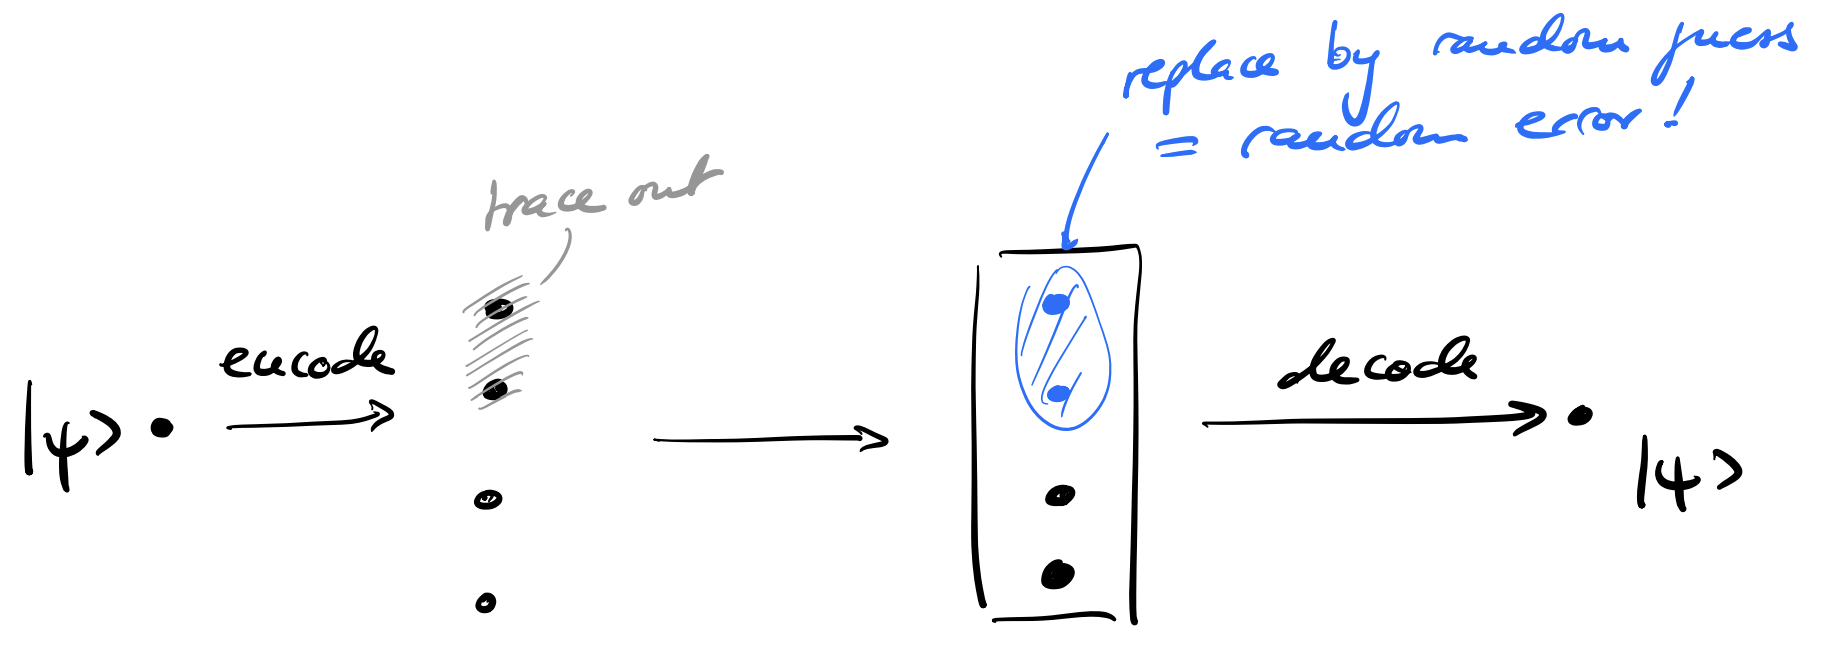
\includegraphics[width=0.8\textwidth]{image-4-1.png}
    \end{center}
    Based on that:
    \begin{center}
      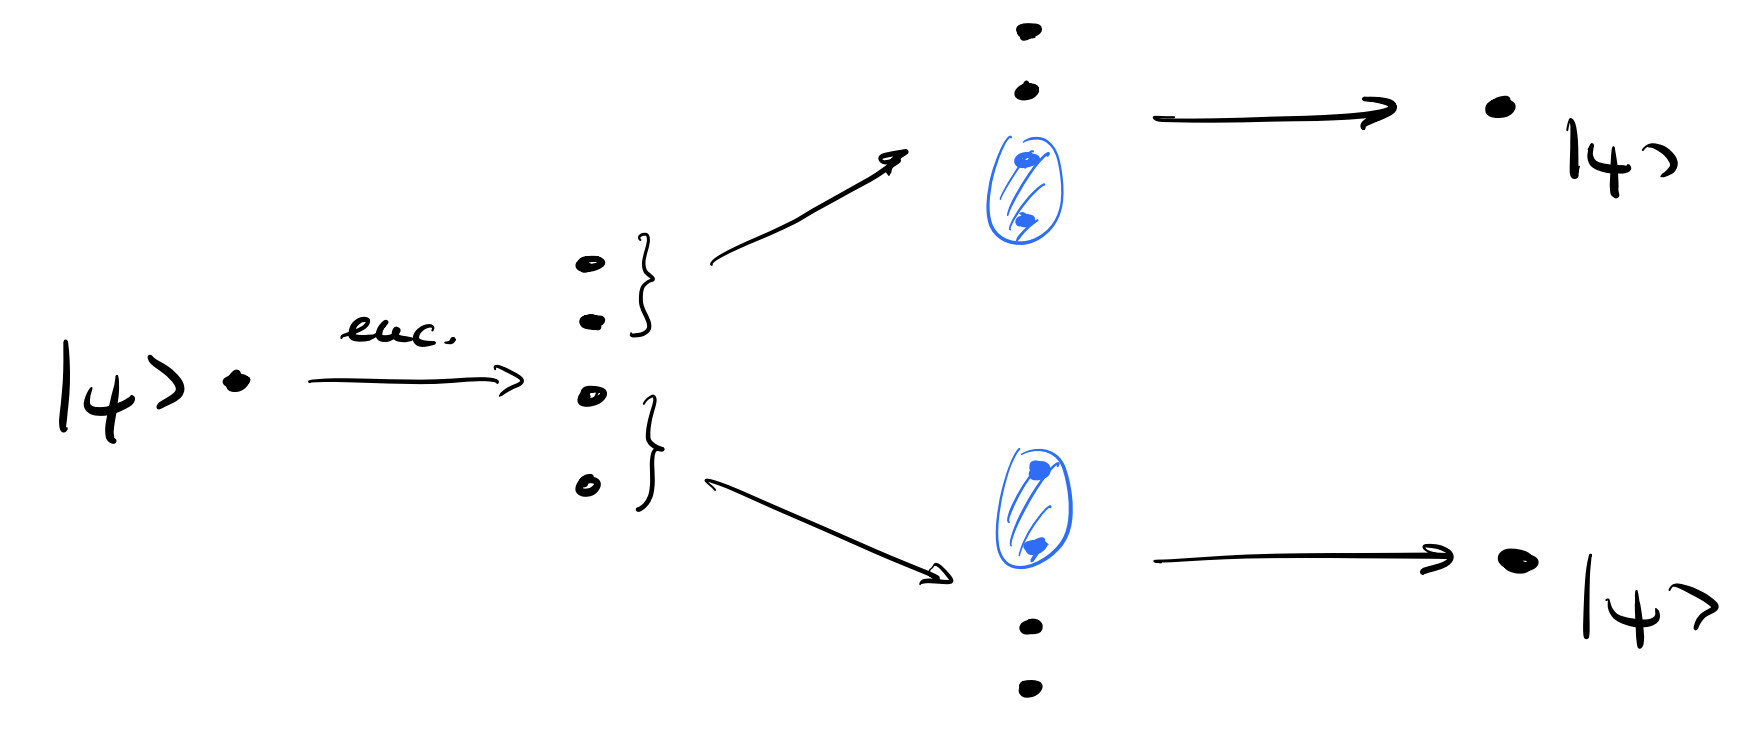
\includegraphics[width=0.8\textwidth]{image-4-2.png}
    \end{center}

    \textbf{\Lightning \, have built a quantum cloner!}

    $\Longrightarrow$ No $[[4,1,3]]$ code can exist, a $[[5,1,3]]$  code would be optimal!
  \end{proof}
\end{example}

\end{document}